% Generated by fig_hero.py; edit the script, not this file.
\documentclass[border=0pt]{standalone}
\usepackage[T1]{fontenc}
\usepackage{times}
\usepackage{textcomp}
\usepackage{amsmath}
\usepackage{graphicx}
\usepackage{tikz}
\graphicspath{{../teaser/}}
% Written by scafig.py; the same palette as the matplotlib figures.
\definecolor{scaInk}{HTML}{1F2328}
\definecolor{scaMid}{HTML}{5B6570}
\definecolor{scaRule}{HTML}{C3C9CF}
\definecolor{scaGrid}{HTML}{E6E9EC}
\definecolor{scaGlobal}{HTML}{2F6DB3}
\definecolor{scaGlobalLight}{HTML}{DCE7F3}
\definecolor{scaLocal}{HTML}{E08A2B}
\definecolor{scaLocalLight}{HTML}{F9E6D0}
\definecolor{scaAccent}{HTML}{13865F}
\definecolor{scaAccentLight}{HTML}{D7EEE4}
\definecolor{scaNeutral}{HTML}{F4F1EA}
\definecolor{scaZoom}{HTML}{FFC21A}
\definecolor{scaLoss}{HTML}{B85C00}
\definecolor{scaArea}{HTML}{7A4EA3}
\definecolor{scaAreaLight}{HTML}{E9E0F1}
\definecolor{scaFull}{HTML}{9AA3AC}

\definecolor{scaZoomB}{HTML}{38C6F4}
\newcommand{\tagfont}{\fontsize{6.5}{7.8}\selectfont\color{scaMid}}
\begin{document}
\begin{tikzpicture}[x=1in,y=1in,
  halo/.style={draw=black,draw opacity=0.35,line width=1.15pt},
  zoombox/.style={line width=0.55pt},
  zoomframe/.style={line width=0.8pt},
  cropframe/.style={line width=0.5pt},
  tabrule/.style={draw=scaRule,line width=0.4pt},
  badge/.style={fill=black,fill opacity=0.58,text opacity=1,text=white,rounded corners=1.2pt,
                inner xsep=1.8pt,inner ysep=1.15pt,font=\sffamily\fontsize{6.5}{7}\selectfont},
  head/.style={inner sep=0pt,font=\sffamily\fontsize{8}{9.6}\selectfont,text=scaInk},
  headours/.style={inner sep=0pt,font=\sffamily\bfseries\fontsize{8}{9.6}\selectfont,text=scaAccent},
  lab/.style={inner sep=0pt,font=\sffamily\fontsize{6.5}{7.8}\selectfont,text=scaMid},
  labhead/.style={inner sep=0pt,font=\sffamily\fontsize{8}{9.6}\selectfont,text=scaInk},
  prompt/.style={inner sep=0pt,align=left,font=\sffamily\itshape\fontsize{6.5}{7.7}\selectfont,text=scaMid},
  val/.style={inner sep=0pt,font=\sffamily\fontsize{7}{8.4}\selectfont,text=scaInk},
  legend/.style={inner sep=0pt,font=\sffamily\fontsize{6.5}{7.8}\selectfont,text=scaMid},
  ]
\useasboundingbox (0,0) rectangle (5.5000,-3.1480);
\node[anchor=north west,inner sep=0pt] at (0.0000,0.0000) {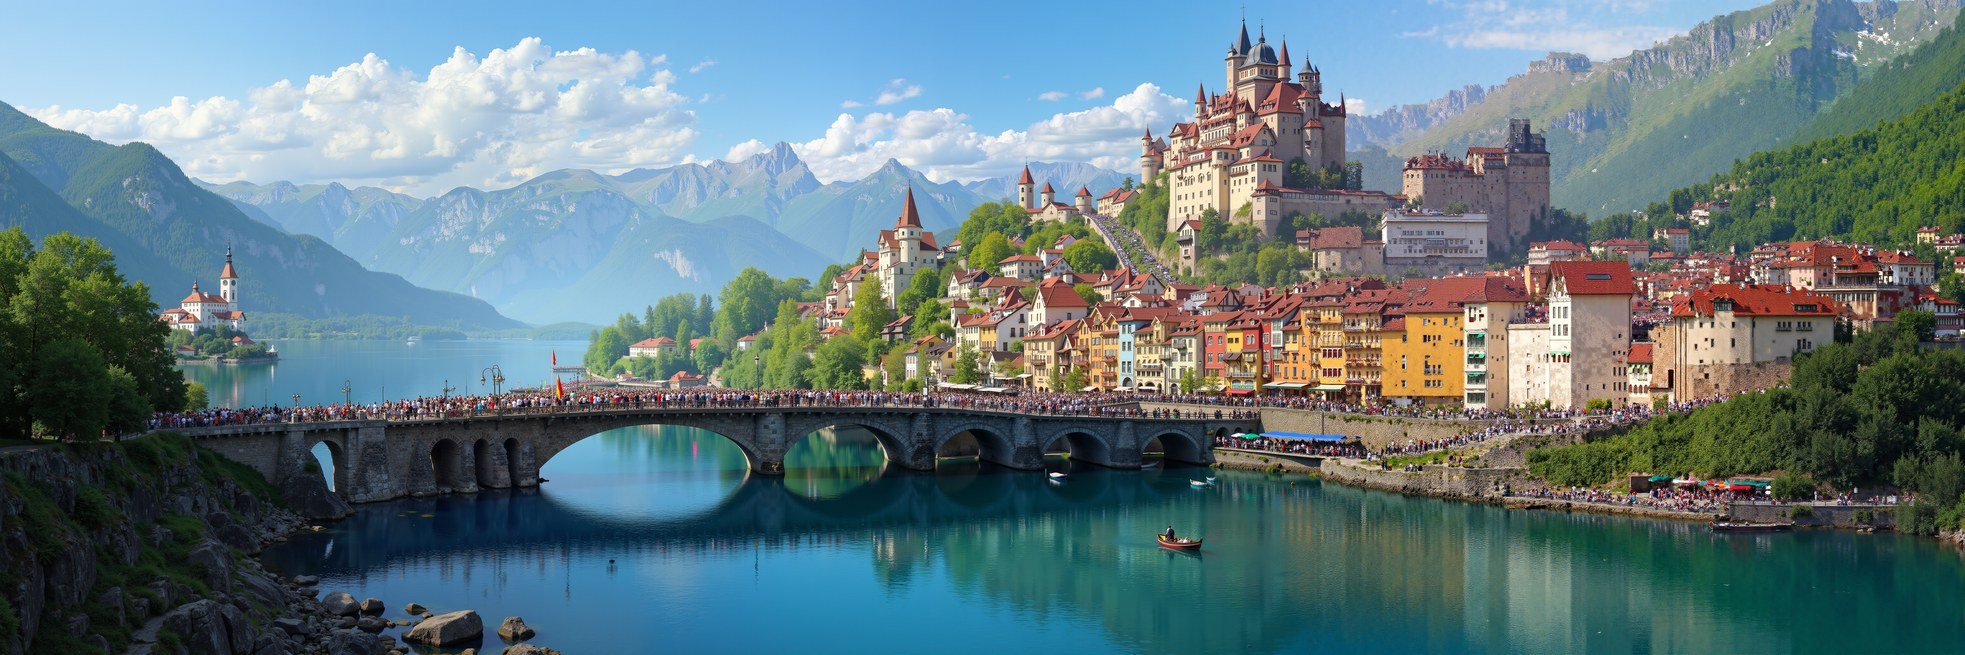
\includegraphics[width=3.2130in,height=1.0710in]{pano.jpg}};
\node[anchor=north west,inner sep=0pt] at (3.2580,-0.0000) {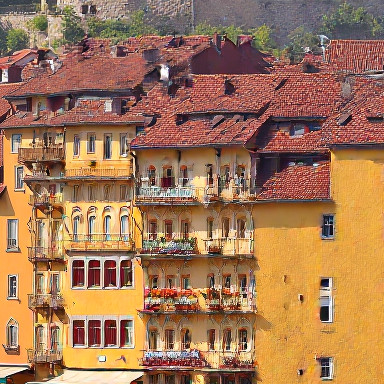
\includegraphics[width=0.5130in,height=0.5130in]{pano_zoom1.jpg}};
\draw[halo] (2.1253,-0.4351) rectangle (2.3261,-0.6359);
\draw[zoombox,draw=scaZoomB] (2.1253,-0.4351) rectangle (2.3261,-0.6359);
\draw[zoomframe,draw=scaZoomB] (3.2580,-0.0000) rectangle (3.7710,-0.5130);
\node[anchor=north west,inner sep=0pt] at (3.2580,-0.5580) {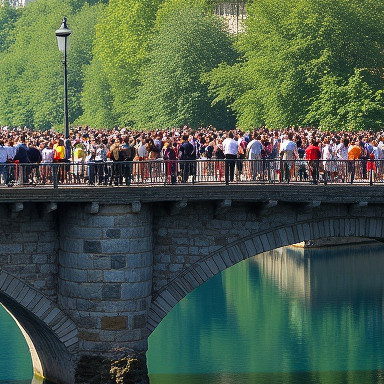
\includegraphics[width=0.5130in,height=0.5130in]{pano_zoom2.jpg}};
\draw[halo] (1.2049,-0.5690) rectangle (1.4057,-0.7698);
\draw[zoombox,draw=scaZoom] (1.2049,-0.5690) rectangle (1.4057,-0.7698);
\draw[zoomframe,draw=scaZoom] (3.2580,-0.5580) rectangle (3.7710,-1.0710);
\node[badge,anchor=north west] at (0.0200,-0.0200) {2048\,$\times$\,6144};
\node[anchor=north west,inner sep=0pt] at (3.8710,0.0000) {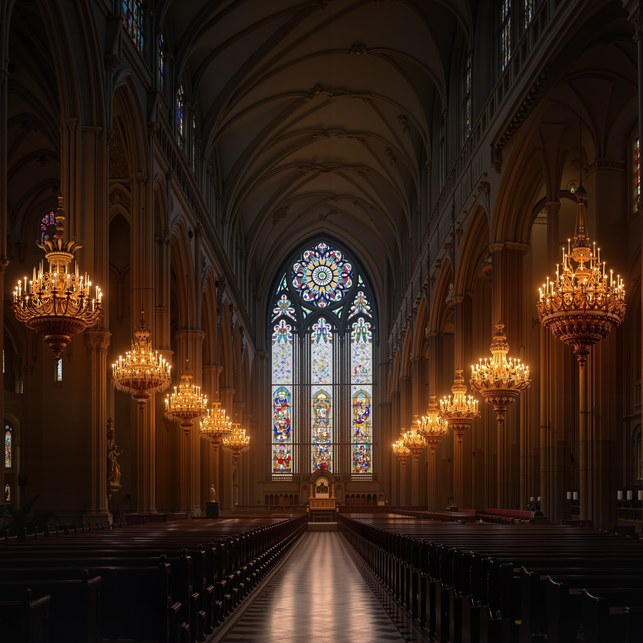
\includegraphics[width=1.0710in,height=1.0710in]{square.jpg}};
\node[anchor=north west,inner sep=0pt] at (4.9870,-0.0000) {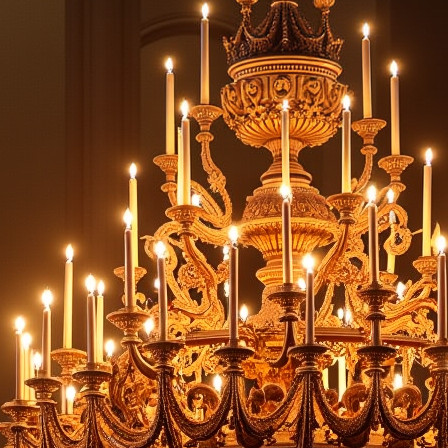
\includegraphics[width=0.5130in,height=0.5130in]{square_zoom1.jpg}};
\draw[halo] (4.7652,-0.3974) rectangle (4.8824,-0.5146);
\draw[zoombox,draw=scaZoomB] (4.7652,-0.3974) rectangle (4.8824,-0.5146);
\draw[zoomframe,draw=scaZoomB] (4.9870,-0.0000) rectangle (5.5000,-0.5130);
\node[anchor=north west,inner sep=0pt] at (4.9870,-0.5580) {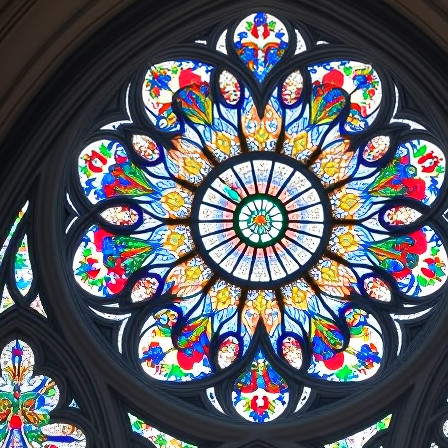
\includegraphics[width=0.5130in,height=0.5130in]{square_zoom2.jpg}};
\draw[halo] (4.3396,-0.4016) rectangle (4.4567,-0.5188);
\draw[zoombox,draw=scaZoom] (4.3396,-0.4016) rectangle (4.4567,-0.5188);
\draw[zoomframe,draw=scaZoom] (4.9870,-0.5580) rectangle (5.5000,-1.0710);
\node[badge,anchor=north west] at (3.8910,-0.0200) {4096\,$\times$\,4096};
\node[anchor=north west,inner sep=0pt] at (1.0800,-1.2360) {
\includegraphics[width=0.6950in,height=0.6950in]{strip_full_full.jpg}};
\node[anchor=north west,inner sep=0pt] at (1.0800,-1.9610) {
\includegraphics[width=0.6950in,height=0.6950in]{strip_full_crop.jpg}};
\draw[halo] (1.3623,-1.4749) rectangle (1.4927,-1.6052);
\draw[zoombox,draw=scaZoom] (1.3623,-1.4749) rectangle (1.4927,-1.6052);
\draw[cropframe,draw=scaZoom] (1.0800,-1.9610) rectangle (1.7750,-2.6560);
\node[head,anchor=base] at (1.4275,-1.1860) {Full attention};
\node[val,anchor=base] at (1.4275,-2.7740) {28};
\node[val,anchor=base] at (1.4275,-2.8820) {186.5\,\,{\tagfont clean}};
\node[val,anchor=base] at (1.4275,-2.9900) {\textminus 2.18\,/\,7.61};
\node[anchor=north west,inner sep=0pt] at (1.8250,-1.2360) {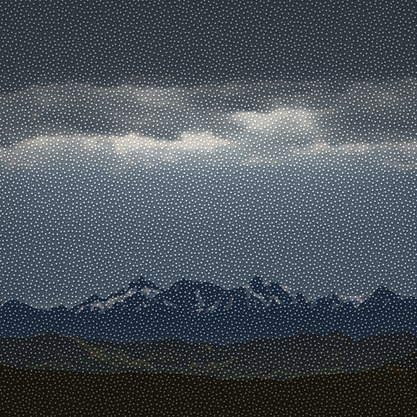
\includegraphics[width=0.6950in,height=0.6950in]{strip_dype_full.jpg}};
\node[anchor=north west,inner sep=0pt] at (1.8250,-1.9610) {
\includegraphics[width=0.6950in,height=0.6950in]{strip_dype_crop.jpg}};
\draw[halo] (2.1073,-1.4749) rectangle (2.2377,-1.6052);
\draw[zoombox,draw=scaZoom] (2.1073,-1.4749) rectangle (2.2377,-1.6052);
\draw[cropframe,draw=scaZoom] (1.8250,-1.9610) rectangle (2.5200,-2.6560);
\node[head,anchor=base] at (2.1725,-1.1860) {DyPE};
\node[val,anchor=base] at (2.1725,-2.7740) {28};
\node[val,anchor=base] at (2.1725,-2.8820) {196.1\,\,{\tagfont campaign}};
\node[val,anchor=base] at (2.1725,-2.9900) {\textminus 0.11\,/\,20.52};
\node[anchor=north west,inner sep=0pt] at (2.5700,-1.2360) {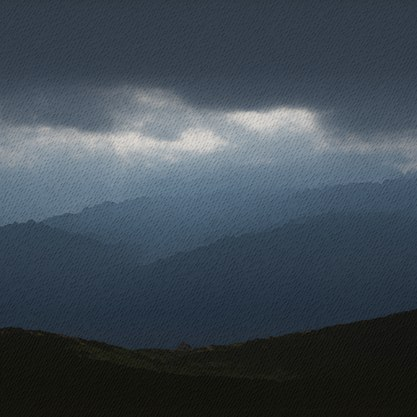
\includegraphics[width=0.6950in,height=0.6950in]{strip_sega_official_full.jpg}};
\node[anchor=north west,inner sep=0pt] at (2.5700,-1.9610) {
\includegraphics[width=0.6950in,height=0.6950in]{strip_sega_official_crop.jpg}};
\draw[halo] (2.8523,-1.4749) rectangle (2.9827,-1.6052);
\draw[zoombox,draw=scaZoom] (2.8523,-1.4749) rectangle (2.9827,-1.6052);
\draw[cropframe,draw=scaZoom] (2.5700,-1.9610) rectangle (3.2650,-2.6560);
\node[head,anchor=base] at (2.9175,-1.1860) {SEGA};
\node[val,anchor=base] at (2.9175,-2.7740) {28};
\node[val,anchor=base] at (2.9175,-2.8820) {190.5\,\,{\tagfont campaign}};
\node[val,anchor=base] at (2.9175,-2.9900) {0.55\,/\,24.37};
\node[anchor=north west,inner sep=0pt] at (3.3150,-1.2360) {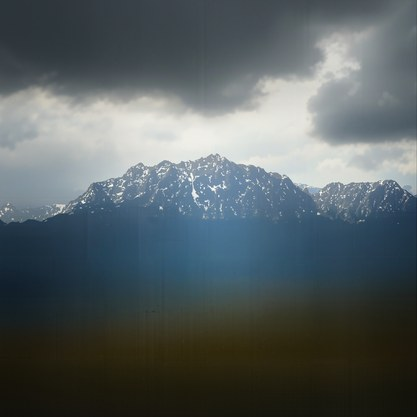
\includegraphics[width=0.6950in,height=0.6950in]{strip_area_full.jpg}};
\node[anchor=north west,inner sep=0pt] at (3.3150,-1.9610) {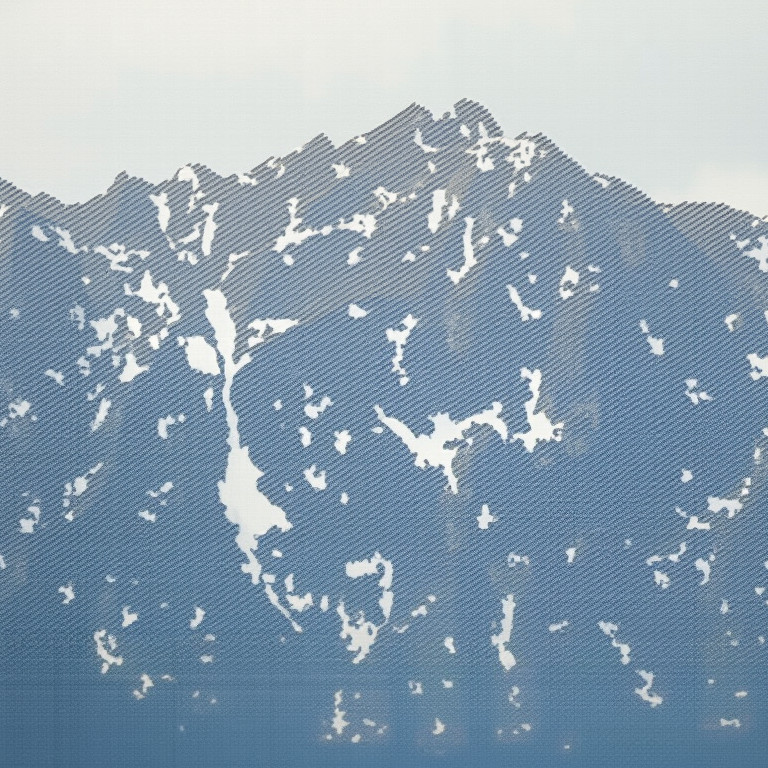
\includegraphics[width=0.6950in,height=0.6950in]{strip_area_crop.jpg}};
\draw[halo] (3.5973,-1.4749) rectangle (3.7277,-1.6052);
\draw[zoombox,draw=scaZoom] (3.5973,-1.4749) rectangle (3.7277,-1.6052);
\draw[cropframe,draw=scaZoom] (3.3150,-1.9610) rectangle (4.0100,-2.6560);
\node[head,anchor=base] at (3.6625,-1.1860) {AReA};
\node[val,anchor=base] at (3.6625,-2.7740) {28};
\node[val,anchor=base] at (3.6625,-2.8820) {202.4\,\,{\tagfont clean}};
\node[val,anchor=base] at (3.6625,-2.9900) {0.92\,/\,27.20};
\node[anchor=north west,inner sep=0pt] at (4.0600,-1.2360) {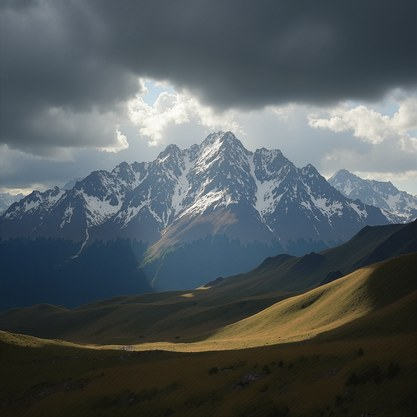
\includegraphics[width=0.6950in,height=0.6950in]{strip_ultraimage_full.jpg}};
\node[anchor=north west,inner sep=0pt] at (4.0600,-1.9610) {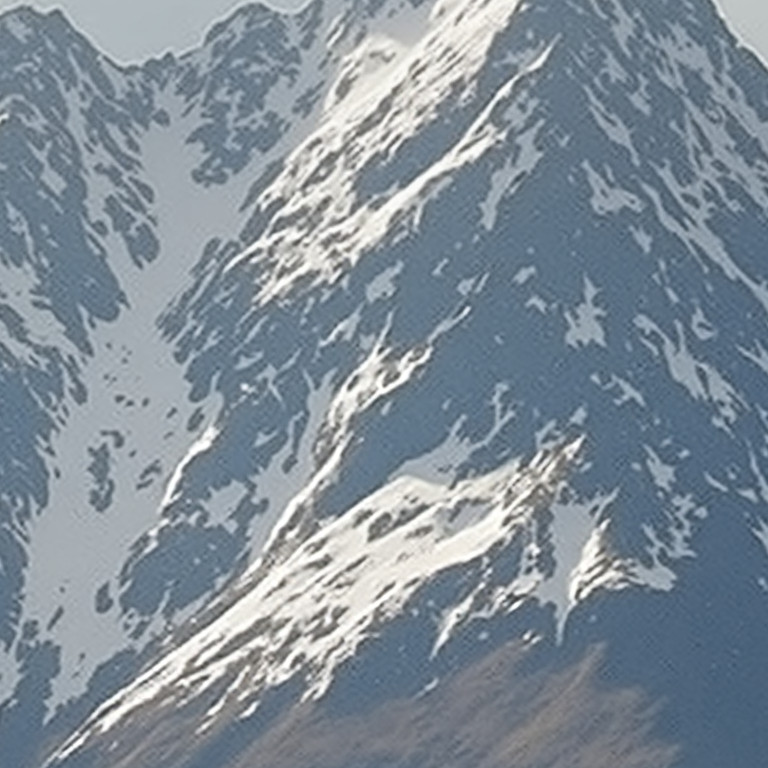
\includegraphics[width=0.6950in,height=0.6950in]{strip_ultraimage_crop.jpg}};
\draw[halo] (4.3423,-1.4749) rectangle (4.4727,-1.6052);
\draw[zoombox,draw=scaZoom] (4.3423,-1.4749) rectangle (4.4727,-1.6052);
\draw[cropframe,draw=scaZoom] (4.0600,-1.9610) rectangle (4.7550,-2.6560);
\node[head,anchor=base] at (4.4075,-1.1860) {UltraImage};
\node[val,anchor=base] at (4.4075,-2.7740) {30+30};
\node[val,anchor=base] at (4.4075,-2.8820) {308.5\,\,{\tagfont campaign}};
\node[val,anchor=base] at (4.4075,-2.9900) {\textbf{1.28}\,/\,\textbf{30.80}};
\node[anchor=north west,inner sep=0pt] at (4.8050,-1.2360) {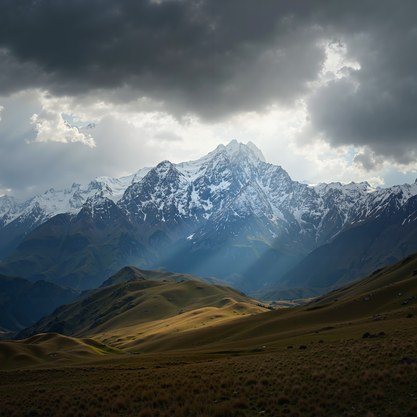
\includegraphics[width=0.6950in,height=0.6950in]{strip_sca_nb_full.jpg}};
\node[anchor=north west,inner sep=0pt] at (4.8050,-1.9610) {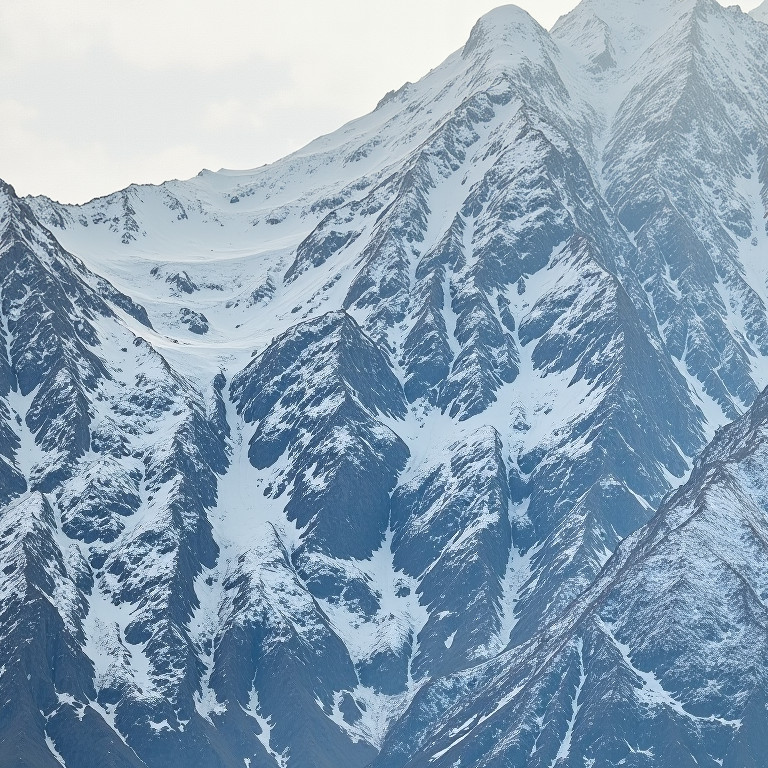
\includegraphics[width=0.6950in,height=0.6950in]{strip_sca_nb_crop.jpg}};
\draw[halo] (5.0873,-1.4749) rectangle (5.2177,-1.6052);
\draw[zoombox,draw=scaZoom] (5.0873,-1.4749) rectangle (5.2177,-1.6052);
\draw[cropframe,draw=scaZoom] (4.8050,-1.9610) rectangle (5.5000,-2.6560);
\node[headours,anchor=base] at (5.1525,-1.1860) {SCA (ours)};
\node[val,anchor=base] at (5.1525,-2.7740) {28};
\node[val,anchor=base] at (5.1525,-2.8820) {\textbf{\color{scaAccent}71.1}\,\,{\tagfont clean}};
\node[val,anchor=base] at (5.1525,-2.9900) {1.23\,/\,29.71};
\node[labhead,anchor=base west] at (0.0000,-1.1860) {Prompt};
\node[prompt,text width=0.9800in,anchor=north west] at (0,-1.2310) {\hyphenpenalty=10000 ``Dramatic mountain landscape under dark, cloud-covered skies, with snow-capped peaks and patches of sunlight illuminating grassy fields and rolling hills.''};
\node[lab,anchor=east] at (1.0200,-2.3085) {768$^2$ crop, 1:1};
\node[lab,anchor=base east] at (1.0200,-2.7740) {Steps};
\node[lab,anchor=base east] at (1.0200,-2.8820) {Time (s)};
\node[lab,anchor=base east] at (1.0200,-2.9900) {ImageReward / HPSv2.1};
\draw[tabrule] (0,-2.6840) -- (5.5000,-2.6840);
\draw[tabrule] (0,-3.0300) -- (5.5000,-3.0300);
\node[legend,anchor=base west] at (0.0000,-3.1230) {\textbf{clean}: batch-1 median of three after warm-up, idle GPU;\enspace \textbf{campaign}: mean over the 191-prompt run, shared nodes.\enspace HPSv2.1 is $\times$100.};
\end{tikzpicture}
\end{document}
